\begin{figure}[h!tb]
\centering
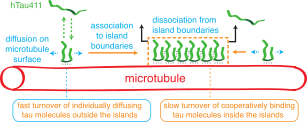
\includegraphics[scale=1]{Figures/tau8.png}
\caption[Schematic representation of island formation.]{
\textbf{Schematic representation of island formation.} Tau molecules bind and unbind with high rates to microtubules, on which they diffuse (fast turnover). When encountering an island (dashed orange box), tau molecules cooperatively associate with the island at its boundaries, rendering the tau molecules stationary, decreasing their unbinding rate (slow turnover), and causing the island to grow in size laterally. Tau molecules from solution can only bind to the inside of an island via displacement of an island-associated tau molecule, resulting in the observed concentration-dependent turnover of tau inside islands. After removal of tau from solution, tau molecules dissociate from the island boundaries, making the island shrink in size laterally.
	}\label{tau8}
\end{figure}
In our investigation of tau interactions with microtubules, we have unveiled the existence of two distinct binding modes of tau to the microtubule. While the diffusive binding mode was already known, our key contribution is the discovery of the cooperative binding mode which results in the formation of cohesive tau islands. Our findings, coupled with complementary work by \cite{tan2019microtubules}, paint a detailed picture of tau's multifaceted behavior on microtubules.
The cooperative binding mode results in a population of stationary tau molecules characterized by remarkably low turnover rates. This is in contrast to the diffusive mode, where tau molecules exhibit high turnover rates. At physiological concentrations, these two distinct populations coexist on the microtubule surface. It is possible that these islands have not yet been described is because the rapidly turning over tau has the potential to mask the underlying island structures, adding a layer of complexity to the visualization and study of these formations \aref{tau8}{}. \par
Our experiments revealed a characteristic density within tau islands of approximately 0.26 tau molecules per tubulin dimer. This consistent density strongly suggests the formation of an ordered monolayer, likely involving all four microtubule-binding repeats of tau, given that a recent cryo-electron microscopy study has shown tau-microtubule binding in such a configuration \parencite{Kellogg2018}. It bears noting that the diffusive, rapidly turning over tau population likely is too elusive to detect in these structural studies due to its transient and fast-moving nature. In addition, this type of binding may reflect the intrinsically disordered nature of tau, and thus not result in any favored binding conformations where an averaging of multiple binding events would lead to an increase in resolution.\par 
The integrity of tau islands appears to hinge on cooperative interactions between the constituent molecules. This cooperativity could stem from direct tau-tau interactions, a hypothesis supported by previous studies demonstrating tau's propensity for liquid-liquid phase separation \parencite{HERNANDEZVEGA20172304} and its ability to form neurofibrillary tangles when hyperphosphorylated \parencite{iqbal2016tau}. Alternatively, or perhaps additionally, this cooperativity might arise from local tau-induced impacts on the microtubule lattice. Such modifications could conceivably translate along the microtubule lattice to adjacent binding sites, thereby enhancing the affinity for incoming tau molecules. This possibility is supported by our observations regarding the behavior of tau within regions of high microtubule curvature. Within these regions, in contrast to surrounding regions, we observed tau binding to persist after tau had been removed from solution, a characteristic it shared with tau molecules within tau islands. I had thus hypothesized that tau islands may require a specific spacing of tubulin dimers to accommodate a proper binding of all microtubule binding repeats. This spacing, I hypothesized, was given both in the case of high-curvature regions as well as in islands. 
\begin{itemize}
    \item In the case of islands, a favorable MT region would at first allow for island nucleation, upon which these initial tau molecules would change the spacing of tubulin dimers in their vicinity, allowing for additional tau molecules to bind, leading to island growth.
    \item  In the case of high-curvature regions, it is clear that the tubulin dimers are spaced differently than on straightd microtubule regions. In the inside of the curved region, tubulin dimers are closer to each other, while on the outside, dimers are further apart from each other. Thus, if the stationary tau binding mode indeed possesses a preference for a different lattice spacing than given on a (undecorated) straight microtubule, it appears likely that this binding mode does occur on some parts of curved microtubules. Importantly, this type of stationary binding would not require any cooperative behavior, and would even preclude such cooperative binding and its concomitant shielding of the microtubule from katanin severing, as we had observed, see e.g. \aref{taucurve}{F-H} (given mechanical constraints set by the microtubule and the antibodies it is bound to, though we did frequently observe tau islands to straighten curved microtubule regions). 
\end{itemize}
Indeed, this hypothesis was confirmed in a follow-up study by my former colleague Valerie Siahaan and collaborators, who found that the cooperative tau binding mode compresses the microtubule lattice \parencite{siahaan2022microtubule}. It is tempting to speculate that the absence of tau from highly curved microtubules \textit{in vivo} may fulfill a regulatory purpose by allowing for a katanin-mediated removal of ill-positioned microtubules. Todo In this respect, it should be noted that another intrinsically disordered MAP, doublecortin, has already been shown to both bind to microtubules cooperatively and bind to curved microtubule regions as well \parencite{Bechstedt2012, Bechstedt2014}. \par

Another intriguing observation from our study was that tau unbinding from islands increases with rising tau concentration in solution. Importantly, this phenomenon cannot be attributed solely to the rapidly turning over tau pool that co-localizes with islands at elevated concentrations. At 20 nM and 100 nM tau, this pool accounts for only approximately 20\% and 40\% of the total tau in the islands, respectively, while the average unbinding time drops by two orders of magnitude. We propose that this concentration-dependent unbinding results from the multivalent attachment of island-incorporated tau, mediated by its four microtubule-binding repeats and potential tau-tau interaction sites. Such concentration-dependent unbinding mechanism has been previously reported for other multivalently interacting macromolecules, in the case of microtubules as well as DNA \parencite{lanskydiffusible2015, sing2014multiple}. Specifically, our model suggests that the multiple interaction sites undergo transient cycles of unbinding and rebinding. At low tau concentrations, transiently released bonds are likely reestablished as partially-bound tau molecules remain anchored to the microtubule by their persisting binding sites. However, with increasing tau concentration in solution, it becomes increasingly probable that a binding site of a solution-phase tau molecule establishes a bond to a temporarily-vacated binding site on the microtubule. This process could sequentially replace an island-incorporated tau molecule, one bond at a time. Similarly, a step-by-step displacement mechanism could also be at play in the case of kinesin-8-driven island disassembly.\par

All of the above points, the consistent density of islands, of 0.26 tau molecules per tubulin dimer, the (now-confirmed) dependence of the cooperative binding mode on a specific lattice constant (Todo) as well as the concentration-dependence of tau unbinding from island regions hint at an integral role of the microtubule binding repeats in the cooperative binding mode. Our (not-yet-published) findings regarding the ionic strength dependence of island stability \pref{tausalt}{} provide further support for the involvement of microtubule binding repeats in cooperative binding. We observed optimal stability at 75mM KCl, suggesting a delicate balance between hydrophobic interactions, likely mediated by the repeats, and ionic interactions. The stronger diffusive mode at 0mM KCl implies a predominance of ionic bonds in this binding mode. These ionic strength dependencies could also explain the varying stationarity of tau molecules within islands at different KCl concentrations. At lower KCl concentrations, single tau molecules within islands were less stationarily bound, potentially switching binding modes more frequently and often having only a subset of their microtubule binding repeats engaged.\par

Our results suggest another intriguing avenue for further research: The interplay between tau islands and motor proteins like kinesin-8 (Kip3), as it presents a potential regulatory mechanism. For example, we can envision cycles of island growth, Kip3 traffic jam formation at island boundaries, eventual overwhelming and disassembly of the island by Kip3, propagation of the traffic jam as a high-density "pulse" along the microtubule, followed by island regrowth and repetition of the process. This dynamic interplay could potentially result in pulsatile Kip3 movement along axonal microtubules, adding another layer of complexity to cellular transport regulation.\par


Finally, the comparatively high tau island nucleation rate right after flushing in tau \pref{tauGROW}{G} implies that some microtubule regions are more suitable for the nucleation of tau islands than others. This could be due to mechanical constraints related for instance to where a given microtubule is tied to the coverslip surface via an antibody. Another determinant of island growth could be post-translational tubulin modifications. Thus, tau island formation may potentially serve as a readout of such modifications, which would in effect allow to amplify the impact of such modifications given the distinct and striking interaction patterns of tau islands with other MAPs. Furthermore, the potential for other intrinsically disordered proteins to form similar cohesive structures on microtubules could add another dimension to MAP sorting and regulation \parencite{Monroy2018}.
The implications of these findings extend to neurodegenerative diseases, where alterations in tau's ability to form islands, possibly due to hyperphosphorylation, could trigger various downstream pathophysiological effects. Todo: Indeed, this was recently confirmed. 
